\section{Computer Experiments} \label{ch:computer_experiments}
This section describes the setup and configuration of the computational experiments conducted in this study, and the accompanied results. The first sections provide details on framework, structure and implementations. The following sections describes the experimental design, and the hyperparameters tuned, 
% A configuration is a set of parameters set prior to training. These are often referred to as hyperparameters, 
divided into two sections, one for \acrshort{convlstm}-models and another for \acrshort{ar}-models. All models are evaluated on their ability to reproduce the cloud cover in the period from 2014 including 2018. At the end, the best configuration from each of the statistical model types are evaluated on their ability to perform a 24-hour cloud cover forecast and compared against existing parameterizations in \acrshort{era5}.

\subsection{Framework, Structure and Implementation} \label{sec:structure_and_implementations} \label{sec:framework}
The numerical methods used in this study are described in Chapter \ref{ch:num_methods}. The code is available on GitHub in the project repository named ``MS'' on \href{https://github.com/hannasv/MS}{https://github.com/hannasv/MS}. Instructions for downloading 
reanalysis (ERA5) data using python is provided. 
The dataset, \acrshort{ecc}, is not published because of a licenses on the \acrshort{msg} data. 
%The repository contains everything need to reproduce the results in this study.
%The experiments are conducted in notebooks and the developed modules are stored in the package ``sciclouds''. Descriptions on how to acquire the data (scripts if possible) and project environment is provided to simplify the process.

The code is developed in Python 3.7, a popular language for scientific software development. The source code is stored in the package \textit{sciclouds}, made available on GitHub through the project repository. Developed modules draw inspiration from the structure of \textit{scikit-learn} (\cite{sklearn_api}).
%and the \textit{keras-tuner} (\cite{chollet2015kerastuner}). 
%The \acrshort{convlstm} is implemented %in \textit{keras} (\cite{chollet2015keras})
%using \textit{tensorflow v 2.0} . %The \textit{keras-tuner} is used to automize the hyperparameter search (\cite{chollet2015kerastuner}). 
The \acrshort{convlstm} is implemented using Tensorflow's keras API (\cite{tensorflow2015}) which simplifies many aspects of building and executing machine learning models. To utilize the analytical solution the \acrshort{ar}-models are trained and evaluated using self-implemented modules.
%The \acrshort{ar}-models are trained and evaluated using self implemented modules. The idea was to utilize the analytical solution of the least squares problem. 
%Many regression modules provide a numerical solution, not the analytical. 
The python package ``sciclouds'' provides a self-implemented version of \acrshort{ar}-models, using the analytical solution to the least squares problem derived in Section \ref{sec:ARmodels}.

Visualizations are generated using \textit{Matplotlib} (\cite{matplotlib}),  \textit{Seaborn} (\cite{seaborn}) and maps using the package \textit{Cartopy} (\cite{Cartopy}). Other illustrations are developed using TIkZ, a language used for producing technical illustrations within the environment of LaTeX.

The package versions are documented in the \textit{requirements.txt} and the project environment called ``sciclouds'' is ready for installation. This is a conda environment, the yaml-file lists the Python packages and requirements necessary for running this code. Below you find the code example for cloning the project and installing the environment.

% Included in the readme file on github. 
\begin{verbatim}
git clone https://github.com/hannasv/MS.git
cd MS
conda env create -f environment.yml
conda activate sciclouds
python setup.py install # installing package from source
\end{verbatim}

Supplementary material for remapping satellite data and filtering masks is available in the supplementary repository \href{https://github.com/hannasv/MS-suppl}{https://github.com/hannasv/MS-suppl}. %To make use of all the functionality available trought ``MS'', the supplementary repository needs to be cloned in the same directory.
The filters are generated from within the environment of PyAEROCOM (\cite{pyaerocom}). 


%Complex computations will cause memory growth, dependant on how many intermediate computations it needs to store. This is the case for \acrshort{convlstm}. To speed up the development process the software is developed on a subset of \acrshort{ecc}. Small adjustments needs to be made, running experiments on the entire data. For instance threads deadlock when extracting large amounts of data. This is a precautionary measure to avoid overloading the system. \textbf{Possible to develop code to do Hyperparameter tuning based on }
%For a more detailed description please see the project repository described in Section \ref{sec:structure_and_implementations}.

\subsection{Hardware} \label{sec:hardware}
%How to deal with big datasets that will easily eat up you memory? ``Big data'' involve processing large amounts of data that does not fit into memory. Processing substantial amounts of data require expert knowledge about distributed systems and analysing for system bottlenecks.  %Although theoretically fascinating it remains to see if \acrshort{convlstm} provide a clear practical advantage over the autoregressive models.
%Conducting experiments on big datasets require external computational resources.  
The experiments described below, are conducted on a 
%This study had access to a 
DGX-2 system consisting of 16 NVIDIA Tesla V100 GPUs, each of 32Gb local memory and 1.5Tb shared memory. %The resources was available through the \acrfull{ex3} project hosted at Simula. 
%This study was awarded access to 1 GPU and 1024G part of the memory. 
The data is stored on a \acrfull{rdma} accessed over Infiniband. %\textit{The best choice of collective implementation depends upon the number and kind of \acrshort{gpu}s, and the network interconnect in the cluster.} 
The DGX-2 system is designed for a high level concurrency and scheduling workers competing for system resources.
%The hardware sets the limitations for efficiency of pipelines and training procedure. 
%\textit{NVIDIA V100 GPU -- The eX3 infrastructure includes a DGX-2 system consisting of 16 NVIDIA Tesla V100 GPUs, allowing simultaneous communication between all eight GPU pairs at 300 GBps through the 12 integrated NVSwitches. This gives a theoretical system-wide system bi-directional  bandwidth of 2.4 TBps. All GPUs have 32 GB of local memory (total of 512 GB) and share a 1.5 TB main memory. The total system has 81,920 CUDA cores, and 10,240 Tensor cores delivering 2 Petaflops of tensor performance. The peak performance in double precision is 125 Teraflops.}
%Working on such a monstrosity pose additional challenges related to porting existing code and virtual environments, developing and debugging code. To eventually end up with an%a achieved 
%acceptable level of efficiency and reliability. \textbf{må de siteres? (\cite{ex3docs} and \cite{ex3homepage}).} 
\begin{table}[ht]
    \centering
    \begin{tabular}{c|c}
        Device &  Type  \\ \hline
        GPU & Tesla V100-SXM3-32GB \\
        CPU & DualProcessor AMD Epyc7601 (SMT2) w/2TB ram and 4TB NVMe 
    \end{tabular}
    \caption{Hardware specifications for the environment used on \acrshort{ex3}. The operating system is Ubuntu 18.04.4.}
    \label{tab:hardware_ex3}
\end{table}
% In the search for the best model configuration, different combinations of hyperparameters are evaluated based on a metric. This study evaluate models based on \acrfull{mae}, see Section \ref{sec:metrics} for more details.

%For the more complex \acrshort{dl}-models, the choice of architecture (model configuration) can easily overload the system memory resources. 

\subsection{Training, validation and test split}
Gradient methods are at the heart of every machine 
learning algorithms. This type of optimization is based on the principle that the model is continuously evaluated against the validation dataset and weights are adjusted to reduce the loss. This raises the need for two datasets during training. The \acrshort{ar}-models are computed based on an analytical solution and have no need for the extra data set. 

Based on the assumption the most recent partition is most representative for the near future, both models were tested on the period 2014 including 2018. The \acrshort{ar}-model is trained on the period 2004 to 2013, while the \acrshort{convlstm}-model is trained on 2004 to 2011 and validated on 2012 to 2013.

Other notable differences in the input data is related to handling missing values. The \acrshort{ar}-models use shorter sequences, and samples containing missing values are simply removed. The \acrshort{convlstm}-model utilize longer sequences, and missing values are replaced by the out-of-sample value, $c=1.5$. 

\subsection{Autoregressive models (AR)}
In the search for the best model configuration, four hyperparameters have been chosen to tune. These are
% %This could have been done using spaced sampling, attempting lags of 1, 2, 5, 10. The result becomes the same, however for large model there might be some time to save.
\textit{feature scaling of the predictors}, the \textit{inclusion of bias}, \textit{number of lags} and a \textit{potential inclusion of environmental variables}. Varying combinations of these parameters results in the set of models trained in this study. 

The optimization process follow the strategy of the simplest models first followed by a gradual increase in complexity. 
Recall that a \acrshort{ar}-model is composed of 13041 individual regression models, one for each grid box.
More theoretical details can be found in Section \ref{sec:ARmodels}. 

\subsubsection{Feature Scaling} \label{sec:scaling_predictors}
Feature scaling is used to standardize the predictor variables.
\begin{equation} \label{eq:scaling_data}
    \mathbf{x} = \frac{\mathbf{x} - \bar{\mathbf{x}}}{\text{STD}(\mathbf{x})}
\end{equation}
The transformation is computed by applying Equation \eqref{eq:scaling_data} to the predictors, represented by $\mathbf{x}$, $\bar{\mathbf{x}}$ represent its average and STD its standard deviation. The resulting data has a reshaped distribution resembling a standard normal distribution, with zero mean and unit variance. This offers an additional benefit of increased numerical stability. %When applied the predictors is transformed according to the following Equation \ref{eq:scaling_data}. 
%The feature scaling is applied after the partitioning into training and test portions. 

It is important to perform the transformation after the data is split into training and test. The mean and standard deviation should be computed based on the training set and applied to both sets. The model is trained to find relations in transformed data. Consequently the test data need to be transformed before the model can be evaluated. 

The partitioning of datasets prior to the transformation is necessary to avoid a information leak between the test data and the trained model. If it was done differently it would result in an unrepresentative measure on performance.
%\subsubsection{Transforming target} \label{sec:transforming_target}
%A trick to avoid predicting unphysical values is fitting against a transformed target. In this study, the target, \acrfull{cfc} ranges from 0 to 1. By applying the inverse sigmoid transformation, see Equation \eqref{eq:inv_sigmoid} the target takes values from the entire real axis $(-\infty, \infty)$. 
%\begin{equation} \label{eq:inv_sigmoid}
%   \sigma^{-1} \left( x \right) = ln \left(\frac{x}{x - 1 + \epsilon} \right)
%\end{equation}
%In the above equation $\epsilon = 10^{-300}$ is added as a precaution for when $x=1$ and division by zero would occur. This would result in the non-numerical value, $-\infty$. The inverse transformation of this is ordinary sigmoid, see Equation \eqref{eq:sigmoid}. By applying this equation values return to the range between 0 and 1, alleviating predictions of out-of-sample values. The sigmoid function is described in Section \ref{sec:artificial neural networks} in the context of its abilities as an activation function in machine learning models and its graph is displayed in Figure \ref{fig:activation_function_example}.

\subsubsection{Lags and Environmental variables}
The dataset prepared for a particular model is determined by the number of lags and the inclusions of environmental variables (temperature, surface pressure, relative and specific humidity). This controls a models the degrees of freedom. All models are trained either on the full set of environmental variables or none of them. They never appear in isolation. 

Lags describe the number of previous timesteps of \acrshort{cfc} included as a predictors. For example, if the lag is three, $L=3$, then the \acrshort{cfc} is predicted based on the cloud cover for the previous three hours. Utilizing all time steps up to and including three hours back in time.

%%%%%%%%%%%%%%%%%%%%%%%%%%%%%%%%%%%%%%%%%%%%% TRUDE RETTET TIL  HER

\subsubsection{Experimental setup} \label{sec:experiments_ar}
The naming conventions for the \acrshort{ar}-models used in this study $AR_{TB_L}$ or $TR_{TB_L}$. $AR$ or $TR$ describe whether the environmental variables are included in the dataset of not. $TR$ is short for traditional and represents the case when environmental variables are omitted. \acrshort{ar} represents the opposite, their inclusion. B represents bias, T symbolizes that scaling predictors is applied and $L_x$ reveals the number of lags, represented with $x$.  

%This description elaborated in Table \ref{tab:ar_model_config}.
To ease the understanding of the naming convention used, Table \ref{tab:ar_model_config} provide four examples. Applying the following convention, $\times$ denoted not applied, \checked denotes applied.
The hyperparameters bias and transformation of the predictors is mutually exclusive. Applying both have no benefits as the transformation cancels the effect of the bias when subtracting the mean. 
\begin{table}[h]
    \centering
    %\resizebox{\textwidth}{!}{%
    \begin{tabular}{ccccc}
 & \textbf{Feature Scaling} & \textbf{Lag} &\textbf{ Environmental Variables} & \textbf{Bias} \\ \hline
    \multicolumn{1}{c}{\textbf{$TR_{B_1}$}} & $\times$  & 1 & $\times$ & \checked   \\ \hline
    \multicolumn{1}{c}{\textbf{$AR_{B_0}$}} & $\times$  & 0 & \checked  & \checked  \\ \hline
    \multicolumn{1}{c}{\textbf{$AR_{T_1}$}} & \checked  & 1 & \times & \times  \\ \hline
    \multicolumn{1}{c}{\textbf{$AR_{B_4}$}} & $\times$  & 4 & \checked & \checked  \\ \hline
    \end{tabular}%
    %}
    \caption{Example configuration of \acrshort{ar}-models, where $\times$ denoted not applied, \checked denotes applied.}
    \label{tab:ar_model_config}
\end{table}

\subsubsection{Evaluation}
The models are all evaluated using \acrfull{mae} and the \acrshort{ar}-models are optimized to fit the next timestep, not longer sequences. Figure \ref{fig:heatmap_ar_models} shows the performance of all \acrshort{ar}-models included in this study, varying the number of lags on the first axis and the other hyperparameters on the second axis. The score is computed by using Equation \eqref{eq:mae}, and putting the parameters $m = 81$, $n=161$ and $k=43824$. 
\begin{figure}
    \centering
    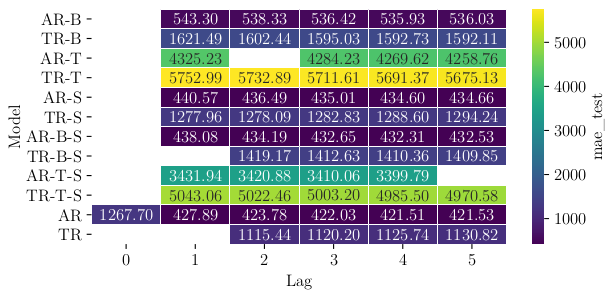
\includegraphics{python_figs/heat_ar_model_mae_test_score.png}
    \caption{Heatmap showing the area averaged test \acrshort{mae} for all the \acrshort{ar}-models included in this work. %$AR-B$ describes the combination of environmental variables and bias, $AR-T$
    }
    \label{fig:heatmap_ar_models}
\end{figure}
%TS: Litt i overkant mange desimaler i denne figuren. Jeg ville ha begrenset meg til 3. Tror det kan være lurt å repetere i caption hva de ulike akronymene betyr, de er litt forvirrende.
With the exception of the $AR-T$-configuration, most models increase most rapidly in performance when adding the first lag. The performance continues to increase for larger numbers of lags, but at a much slower rate. This indicates that the cloud cover at previous timesteps is indeed a useful predictor. The largest variations in performance is caused by varying configurations of $AR$, $B$, $T$ and $TR$. 

%%%%%%%%%%%%%%%%%%%%% Ta for deg alle variablene. 
The configurations employing feature scaling, $T$ have the overall lowest performace. A grid \acrshort{mae} of roughly $0.5$ is high when the target varies in the range from 0 to 1. The inclusion of a bias in combination with $AR$ improves the performance, while for $TR$ it has the opposite effect and decreases the performance. In conclusion, $T$ is not a setting suitable for the cloud forecasting problem.

The $TR$-configuration performs a lot better than $T$, and the set of models have an \acrshort{mae} close to $0.14$. Since $AR$ outperforms $TR$ for all configurations, except for $T$, this indicates that the environmental variables provide useful information. 

Relatively small gain, may still be important, and the skill of the best model, $AR-B-L_5$, is $0.04901$, which is excellent. This shows that there is enough information in the set of environmental variables and previous cloud cover to predict cloud cover one hour into the future.

\subsubsection{Parameterization $\mathbf{AR-B-L_5}$}
%%%%%%%%%%%%%%%%%%%% TEXT ON WEIGHTS 
%Denne seksjonen kunne vel hatt et mer informativt navn?
\begin{figure}
    \centering
    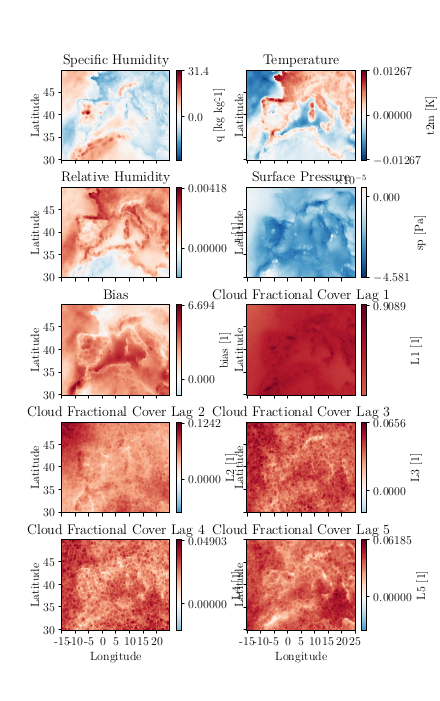
\includegraphics[scale=0.87]{python_figs/weights_AR-B-L5_best_ar_model.png}
    \caption{The weights of the $AR-B-L_5$-model.}
    \label{fig:weights_best_model}
\end{figure}
Figure \ref{fig:weights_best_model} shows the weights in $AR-B-L5$. Note that the colorbars are different for all subplots, but the colors are consistent, with red being positive and blue negative. The \acrshort{ar}-model is a weighted sum over all the variables. Negative input values are unphysical. With the exception of $r$, negative values are not present, as documented in Section \ref{sec:all_stats}. In the case of relative humidity, $r$ they are rarely present, but exist, and the minimum values is $-6.6505$. 
The surface pressure weight is negative for the entire grid. A possible interpretation of this is that higher values of surface pressure will cause large reductions in cloud cover.
%TS: Er det egentlig en tolkning, eller rett og slett bare fakta?
This is in agreement with the cloud physics described in Section \ref{sec:ecc}, stating that areas of high pressure are associated with descending airmasses, which do not lead to cloud formation.

%\textbf{The follwowing statement is true for the remaining variables}
For the other variables, positive values contribute to cloud formation and negative values to dissipation.

By studying the weights of the five hours of previous timesteps, it is clear that they all contribute in producing the predicted cloud cover. $L_1$ have the highest weights, reaching a maximum of 0.9, and is nearly constant over the entire grid. 
In comparison the weights of other lags are small, and this may explain the minor change increasing number of lags, shown in Figure \ref{fig:heatmap_ar_models}. 
%\textbf{This explains the copying effect seen in the sequence plotted.}

The behavior of relative and specific humidity is puzzling. They exhibit the approximately opposite behavior. North Africa has one sign, and Europe has another. In most regions where relative humidity appears to promote clouds, specific humidity appears to reduce the cloud cover. 
The specific humidity has values of $\hat{q}~0.005$ see Figure \ref{fig:all_stats_q} and for relative humidity values are $\hat{r}~75$, which makes them the same order and the weighted sum can potentially cancel. 

In most areas of the European continent temperature is a positive indicator for cloud formation. The temperature weight also shows an opposite spatial distributions compared to that of specific humidity, thereby resembling the weight of relative humidity. 
% Future work undersøke hvordan T SP R er relatert og kanskje redusere antall enviornmental variables litt.
%TS: For forståelsen kunne det nok være bra å se på ulike årstider for seg, så det kan nevnes under future work
\clearpage

\subsection{Convolutional LSTM (ConvLSTM)}
%\textbf{Therefore the tuning of \acrshort{convlstm}-models was done manually. There is a mind-boggling amount of choices for hyperparameters, the initial configuration used in the conducted experiments for this project draw inspiration from this paper by \citeauthor{SunAirLSTM} (\citeyear{SunAirLSTM}).
%The models are described in Section \ref{sec:related_work}.

The formulation of the air quality forecasting problem presented by \citeauthor{SunAirLSTM}, see Section \ref{sec:related_work} is similar to the formulation of the cloud fractional cover forecasting problem presented in this study. This study adopts the machine learning setup in \citepaper{SunAirLSTM}. Manual tuning of the models is applied to avoid a breakdown of the computer caused by too many parameters. When building \acrshort{convlstm} networks, the list of tunable parameters is extensive. These hyperparameters are divided into subsets of tuned and constant parameters.

The following section describes the tuned hyperparameters, batch size, sequence length, number of hidden states and the dimensions of the kernel. The dataset is partitioned into subsets called batches. The batch size is the number of sequences a weight update is based on. Epochs describes the number of times the model loops over the entire dataset. The sequence length is the number of timestamps a model is optimized to learn to predict. The number of hidden states it the number of kernels it learns in each layer. %, see Section \ref{sec:convolutional neural network} for a detailed description of hidden states. %TS: Skal det være "timestamps" over? Eller "timsteps"?
The kernel dimensions determines the number of neighbors influencing an activation. Using kernel 1x1 results in the state-to-state transitions similar to \acrshort{ar}-models by removing interactions between adjacent pixels. A more detailed description on these parameters is provided in Sections \ref{sec:convolutional neural network} to \ref{sec:convolutional_lstm}. 

This section describe the hyperparameters kept constant. Between each \acrshort{convlstm}-layer there is a \acrfull{batchnorm}-layer, implemented using default settings. This type of %TS: her mangler det noen ord
first used by \citepaper{ioffe2015batch} in \acrshort{cnn} and it showed three benefits, the network was less sensitive to the weight initialization, higher learning rate and it did not need dropout. Dropout is another hyperparameter, which randomly removes some of the trained weights to prevent overfitting. This is computationally expensive,so disabling dropout accelerates the training process.
``Padding same'' is applied to all \acrshort{convlstm}-layer, to make sure the input and output dimensions are the same, see Section \ref{sec:padding}. The model returns a sequence and the input sequences are not shuffled. 
%TS: Påfølgende setning er uforståelig
The dimensions of the output layer are completely determined by the task. To produce a cloud cover forecast the output kernel and number of hidden states are put to one.

The weights were initialized based on the scheme ``LeCun uniform''  (\cite{Lecun98efficientbackprop}). Callbacks such as %early stopping was impleme with patience \textbf{forgot to apply this when rerunning the models..} of 10 epochs and 
terminate on NaN's have been applied to avoid prolonged training time. The optimizer ADAM is used with the following settings, $\text{learning rate}=0.001$, $\text{beta1}=0.9$, $\text{beta2}=0.999$, $\text{epsilon}=1e-07$ (\cite{Kingma2015Adam:Optimization}). The default settings in Tensorflow use $\text{epsilon}=1e-08$. The loss function is \acrfull{mse}, and the models are evaluated based on \acrfull{mae}. Both metrics are described in Section \ref{sec:metrics}. 
%The main difference between these functions is that \acrshort{mse} penalize points further away. This has its advantages in training the model, but makes it more difficult to interpret the results. The squared numbers in the range 0 to 1 shrink.
A list of compiled non-trainable architecture are included in the Appendix \ref{app:list_non_trainable_architectures} as a reference for further studies.

\subsubsection{Experimental setup}
Models are given names based on an extension of the convention from \citepaper{precip_nowcasting}.
The batch size and sequence length is included and 
the resulting naming convention is  $ConvLSTM-B_{x}-SL_{y}-\text{hidden states}-filter$\times$filter$. Table \ref{tab:convlstm_config} provide a set of example configurations, here the square brackets list the number of hidden states (or kernels), and the position of the layer. If the bracket has three members the network has three layers. %The idea was to make the convention general enough to allow for varying hidden states and kernels. 

\begin{table}[hp]
    \centering
    \resizebox{\textwidth}{!}{%
    \begin{tabular}{ccccc}
     \textbf{ConvLSTM Model} & \textbf{Sequence Length} & \textbf{Batch Size} & \textbf{Hidden States} & \textbf{Kernels} \\ \hline
    $B_{10}-SL_{24}-16-3\times3-16-3\times3$ & 24 & 10 & [16, 16]   & [3, 3] \\ \hline
    $B_{10}-SL_{24}-32-1\times1-32-1\times1$ & 24 & 10 & [32, 32]  & [1, 1] \\ \hline
    $B_{10}-SL_{24}-32-3\times3-32-3\times3$ & 24 & 10 & [32, 32] & [3, 3] \\ \hline
    $B_{10}-SL_{24}-32-5\times5-32-5\times5$ & 24 & 10 & [32, 32] & [5, 5] \\ \hline
    $B_{10}-SL_{24}-8-3\times3-8-3\times3-8-3\times3$ & 24 & 10 & [8, 8, 8] & [3, 3, 3] \\ \hline
    $B_{5}-SL_{6}-32-3\times3-32-3\times3-32-3\times3$ & 6 & 5 & [32, 32, 32] & [3, 3, 3] \\ \hline
    \end{tabular}%
    }
    \caption{Examples of \acrshort{conv}-model names and their configurations.}
    \label{tab:convlstm_config}
\end{table}

\subsubsection{Evaluation}
The input volume of \acrshort{convlstm}-models are different from the \acrshort{ar}-model, and the axis ``batch'' and ``sequence length'' are merged before the score is computed by using Equation \eqref{eq:mae}, and putting the parameters $m = 81$, $n=161$ and $k=43680$. Note that the $k$ value is a bit smaller than for \acrshort{ar}-models, this is caused by employing the ``drop remainder batch'' during training. 

\begin{figure}
    \centering
    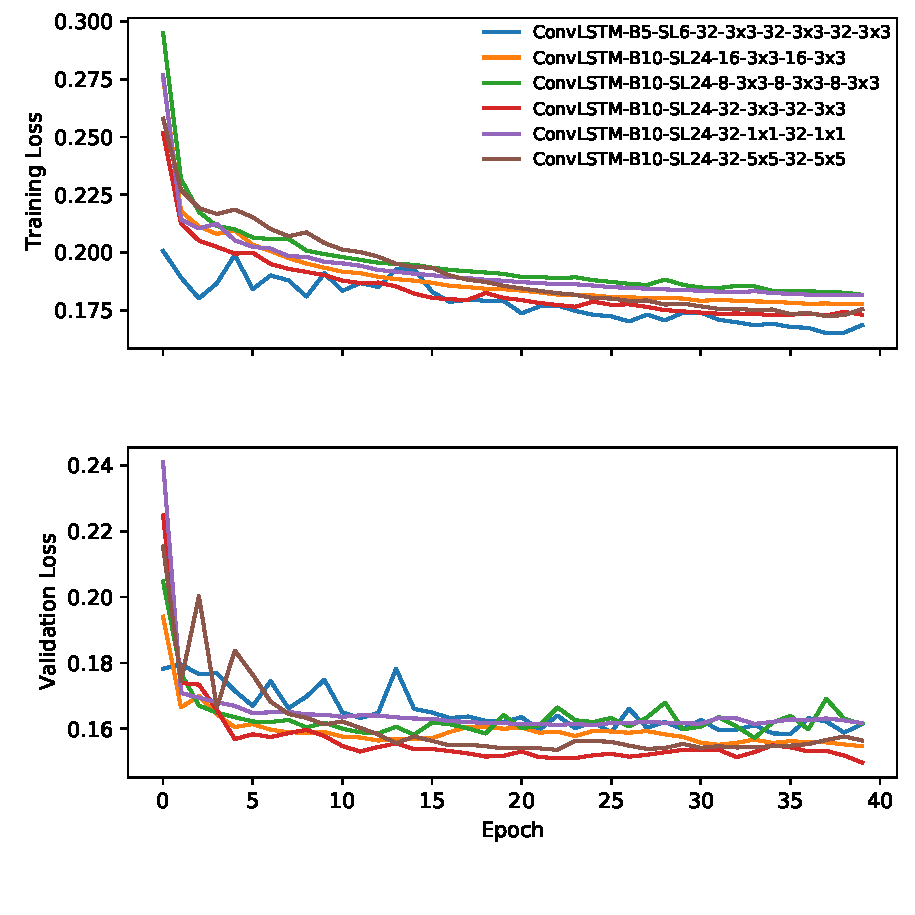
\includegraphics{python_figs/epoch_vs_loss.pdf}
    \caption{The loss of the trained model as a function of epochs.}
    \label{fig:convlstm_loss}
\end{figure}

Figure \ref{fig:convlstm_loss} shows the loss curves in the training process for all the compiled models in this study. As expected, they all ``learn'' the most rapidly in the beginning of the training process. This is shown in the figure as the steep drop in loss between the first and second epoch. 
%\textbf{Note that the training loss is higher than the validation loss since there is a higher number of samples in this set and the loss is not scaled by the number of samples.} 

%%%%%%%%%%%%%%%%%%%%%%%%% The copied dictionary is the result from tf.evaluate. 
\begin{table}[]
    \centering
    \resizebox{\textwidth}{!}{
    \begin{tabular}{c|lccc}
    \textbf{ConvLSTM Model} & \textbf{Train Loss} & \textbf{Val Loss} & \textbf{Test Loss} & \textbf{Num. Params.} \\ \hline 
    $B_{10}-SL_{24}-16-3\times3-16-3\times3$ & 0.1779 & 0.1547 & 0.1575 &  30 296\\ \hline
    % {"loss": 0.15752051770687103, "mean_squared_error": 0.15752056241035461, "r2_keras": 0.15506696701049805, "mean_absolute_error": 0.34570422768592834}

    $B_{10}-SL_{24}-32-1\times1-32-1\times1$ & 0.1817 & 0.1617 & 0.1649 & 13 464 \\ \hline
    % {"loss": 0.1649022251367569, "mean_squared_error": 0.1649022400379181, "r2_keras": 0.1159096509218216, "mean_absolute_error": 0.35085538029670715}
    \rowcolor{red!30}
    $B_{10}-SL_{24}-32-3\times3-32-3\times3$ & 0.1731 & 0.1497 & 0.1534 & 115 864 \\ \hline
    %{"loss": 0.15340088307857513, "mean_squared_error": 0.15340085327625275, "r2_keras": 0.17754235863685608, "mean_absolute_error": 0.33814743161201477}
    
    $B_{10}-SL_{24}-32-5\times5-32-5\times5$ & 0.1755 & 0.1564 & 0.1589 & 320 664 \\ \hline
    % {"loss": 0.15889282524585724, "mean_squared_error": 0.15889279544353485, "r2_keras": 0.147248774766922, "mean_absolute_error": 0.34079509973526}
    
    $B_{10}-SL_{24}-8-3\times3-8-3\times3-8-3\times3$ &  0.1817 & 0.1615 & 0.1634 & 12 920 \\ \hline
    % {"loss": 0.16335555911064148, "mean_squared_error": 0.16335561871528625, "r2_keras": 0.12448494136333466, "mean_absolute_error": 0.3477591276168823}
    
    $B_{5}-SL_{6}-32-3\times3-32-3\times3-32-3\times3$ & 0.1686 & 0.1615  & 0.1633 &  189 848 \\ \hline
    %{"loss": 0.1632702797651291, "mean_squared_error": 0.16327014565467834, "r2_keras": 0.09565786272287369, "mean_absolute_error": 0.3411720395088196}
    
      \end{tabular}
    }
    \caption{Results, metrics and number of parameters for the trained models. The best model \acrshort{convlstm}-model is highlighted in light blue. The loss presented is averaged over on batch, this is the keras default. Since its only used to chose the best model, there is no reason to upscale the numbers.}
    \label{tab:convlstmLoss}
\end{table}
From Figure \ref{fig:convlstm_loss} and Table \ref{tab:convlstmLoss}  it is clear that the best performing \acrshort{convlstm}-model is the $ConvLSTM-B_{10}-SL_{24}-32-3\times3-32-3 \times3$. The run can be seen as the red line in both the table and figure. It has the lowest test and validation loss after 40 epochs, though another model $ConvLSTM-B_{5}-SL_{6}-32-3\times3-32-3 \times3-32-3 \times3$ has a better training loss. As might be deduced based on the similarities in the names, the two models have similar architectures.
The last model has an additional layer, this may have allowed it to learn a better representation on the training data presented, however the skill of predicting on unseen data is most important. The best configuration is therefore $ConvLSTM-B_{10}-SL_{24}-32-3\times3-32-3 \times3$.

In some cases reducing the spatiotemporal resolution can enable the model to learn even more (\cite{precip_nowcasting}). This is arguably not applicable for this task, since cloud cover has an average lifetime of one hour, as mentioned in Section \ref{sec:cloud_in_climate_system}. The reduction can not be applied without most likely producing a significant loss of information.

Comparisons of input data to the works by \citeauthor{precip_nowcasting} (\citeyear{precip_nowcasting}) and \citeauthor{SunAirLSTM} (\citeyear{SunAirLSTM}), has to be done based on input volumes. The dimensions are flattened to generalize the comparison. \citepaper{precip_nowcasting} is trained on $1,629,600,000$ data points, \citepaper{SunAirLSTM} on $28,513,800$ and \acrshort{ecc} on $21,220,315,200$. %Consequently, the models in this study is trained on more than 10 times the amount of data. 
In other words,  this study has trained a \acrshort{convlstm}-model on a much larger amount of data than earlier studies. % How to say that this is harder.

$ConvLSTM-B_{10}-SL_{24}-32-3\times3-32-3 \times3$-model architecture is shown in Figure \ref{fig:best_ml_architecture}. The model consists of three \acrshort{batchnorm} and  \acrshort{convlstm}-layer pairs. Both \acrshort{convlstm} layers have 32 hidden states and a $3\times 3$ kernel. The output layer has one hidden state and the kernel dimension of $1\times 1$. The input shape is $10\times24\times81\times161\times4$ and output $24\times81\times161\times1$. 
\begin{figure}
    \centering
    \begin{tikzpicture}[x={(1,0)},y={(0,1)},z={({cos(60)},{sin(60)})},
font=\sffamily\small,scale=1.9] % 1.7 passer bra på siden.

\tikzset{circle dotted/.style={dash pattern=on .05mm off 2mm,
                                         line cap=round}}

%
% comment these out if you want to see where the axes point to
% \draw[-latex] (0,0,0) -- (3,0,0) node[below]{$x$};
% \draw[-latex] (0,0,0) -- (0,3,0) node[left]{$y$};
% \draw[-latex] (0,0,0) -- (0,0,3) node[below]{$z$};
% a plane
\tikzset{pics/fake box/.style args={% #1=color, #2=x dimension, #3=y dimension, #4=z dimension
#1 with dimensions #2 and #3 and #4}{
code={
\draw[teal,ultra thin,fill=#1]  (0,0,0) coordinate(-front-bottom-left) to
++ (0,#3,0) coordinate(-front-top-right) --++
(#2,0,0) coordinate(-front-top-right) --++ (0,-#3,0) 
coordinate(-front-bottom-right) -- cycle;
\draw[teal,ultra thin,fill=#1] (0,#3,0)  --++ 
 (0,0,#4) coordinate(-back-top-left) --++ (#2,0,0) 
 coordinate(-back-top-right) --++ (0,0,-#4)  -- cycle;
\draw[teal,ultra thin,fill=#1!80!black] (#2,0,0) --++ (0,0,#4) coordinate(-back-bottom-right)
--++ (0,#3,0) --++ (0,0,-#4) -- cycle;
\path[teal,decorate,decoration={text effects along path,text={BATCH NORM}}] (#2/2,{3.4+(#3-2)/2},0) -- (#2/2,0,0);
}
}}
%3.0/1.5, 3.0/3.3, 3.0/5.0
\foreach \X / \Y in {3.0/1.3, 3.0/3., 3.0/4.6} 
%2.2,2.2,2.0
{
\draw pic (box1-\Y) at (\Y,-\X/2,0) {fake box=white!70!teal with dimensions 0.5 and {2*\X} and 1*\X};
}

%%%%%%%%%%%%%%%%%%%%%%%%%%%%%%%%%%%% 
\tikzset{pics/fake box/.style args={% #1=color, #2=x dimension, #3=y dimension, #4=z dimension
#1 with dimensions #2 and #3 and #4}{
code={
\draw[gray,ultra thin,fill=#1]  (0,0,0) coordinate(-front-bottom-left) to
++ (0,#3,0) coordinate(-front-top-right) --++
(#2,0,0) coordinate(-front-top-right) --++ (0,-#3,0) 
coordinate(-front-bottom-right) -- cycle;
\draw[gray,ultra thin,fill=#1] (0,#3,0)  --++ 
 (0,0,#4) coordinate(-back-top-left) --++ (#2,0,0) 
 coordinate(-back-top-right) --++ (0,0,-#4)  -- cycle;
\draw[gray,ultra thin,fill=#1!80!black] (#2,0,0) --++ (0,0,#4) coordinate(-back-bottom-right)
--++ (0,#3,0) --++ (0,0,-#4) -- cycle;
\path[gray,decorate,decoration={text effects along path,text={CONV LSTM}}] (#2/2,{3.4+(#3-2)/2},0) -- (#2/2,0,0);
}
}}

%%%%%%%%%%%%%%%%%%%%%%%%%%%%%%
\foreach \X / \Y in {3.0/1.6, 3.0/3.3, 3.0/4.9}
%2.2,2.2,2.0
{
\draw pic (box1-\Y) at (\Y,-\X/2,0) {fake box=white!70!gray with dimensions 0.5 and {2*\X} and 1*\X};
}

%\foreach \X/\Col in {0.0/red,0.2/green,0.4/cyan, 0.6/yellow, 6.8/blue} %{6.5/red,6.7/green,6.9/blue}
%{\draw[canvas is yz plane at x = \X, transform shape, draw = black, fill = \Col!50!white, opacity = 0.5] (0,0.5) rectangle (2,-1.5);}

%\draw[gray!60,thick] (-0.1,-0.1,-1.6) coordinate (1-1) -- (-0.1,-0.1,0.6) coordinate (1-2) -- (-0.1, 2.,0.6) coordinate (1-3) -- (-0.1, 2.1,-1.6) coordinate (1-4) -- cycle;
%\draw[gray!60,thick] (0.8,-0.1,-1.6) coordinate (2-1) -- (0.8,-0.1,0.6) coordinate (2-2) -- (0.8, 2.,0.6) coordinate (2-3) -- (0.8,2.1,-1.6) coordinate (2-4) -- cycle;

%%%%%%%%%%%%%%%%%%%%%%%%%%%%%%%%%%%% 
\tikzset{pics/fake box/.style args={% #1=color, #2=x dimension, #3=y dimension, #4=z dimension
#1 with dimensions #2 and #3 and #4}{
code={
\draw[gray,ultra thin,fill=#1]  (0,0,0) coordinate(-front-bottom-left) to
++ (0,#3,0) coordinate(-front-top-right) --++
(#2,0,0) coordinate(-front-top-right) --++ (0,-#3,0) 
coordinate(-front-bottom-right) -- cycle;
\draw[gray,ultra thin,fill=#1] (0,#3,0)  --++ 
 (0,0,#4) coordinate(-back-top-left) --++ (#2,0,0) 
 coordinate(-back-top-right) --++ (0,0,-#4)  -- cycle;
\draw[gray,ultra thin,fill=#1!80!black] (#2,0,0) --++ (0,0,#4) coordinate(-back-bottom-right)
--++ (0,#3,0) --++ (0,0,-#4) -- cycle;
\path[gray,decorate,decoration={text effects along path,text={INPUT}}] (#2/2,{2.4+(#3-2)/2},0) -- (#2/2,0,0);
}
}}

%%%%%%%%%%%%%%%%%%%%%%%%%%%%%%
\foreach \X / \Y in {3.0/-1.0}
%2.2,2.2,2.0
{
\draw pic (box1-\Y) at (\Y,-\X/2,0) {fake box=white!70!green with dimensions 2.5 and {2*\X} and 1*\X};
}

\tikzset{pics/fake box/.style args={% #1=color, #2=x dimension, #3=y dimension, #4=z dimension
#1 with dimensions #2 and #3 and #4}{
code={
\draw[gray,ultra thin,fill=#1]  (0,0,0) coordinate(-front-bottom-left) to
++ (0,#3,0) coordinate(-front-top-right) --++
(#2,0,0) coordinate(-front-top-right) --++ (0,-#3,0) 
coordinate(-front-bottom-right) -- cycle;
\draw[gray,ultra thin,fill=#1] (0,#3,0)  --++ 
 (0,0,#4) coordinate(-back-top-left) --++ (#2,0,0) 
 coordinate(-back-top-right) --++ (0,0,-#4)  -- cycle;
\draw[gray,ultra thin,fill=#1!80!black] (#2,0,0) --++ (0,0,#4) coordinate(-back-bottom-right)
--++ (0,#3,0) --++ (0,0,-#4) -- cycle;
\path[gray,decorate,decoration={text effects along path,text={OUTPUT}}] (#2/2,{2.6+(#3-2)/2},0) -- (#2/2,0,0);
}
}}

\foreach \X / \Y in {3.0/6.1}
%2.2,2.2,2.0
{
\draw pic (box1-\Y) at (\Y,-\X/2,0) {fake box=white!70!blue with dimensions 1.0 and {2*\X} and 1*\X};
}

%\foreach \X in {4,1,3}
%{\draw[gray!60,thick] (1-\X) -- (2-\X);}

\node[draw,single arrow, orange,fill=orange!30] at (0.8, 0.5,0) {BATCH};
\node[draw,single arrow, orange,fill=orange!30] at (2.4, 0.5,0) {$3\times 3$};
\node[draw,single arrow, orange,fill=orange!30] at (4., 0.5,0) {$3\times 3$};
\node[draw,single arrow, orange,fill=orange!30] at (5.6, 0.5,0) {$1\times 1$};

%\begin{scope}[on background layer]
%\node[orange,thick,rounded corners,fill=orange!30,fit=(A1) (A3)]{};
%\node[gray,thick,rounded corners,fill=gray!10,fit=(B1) (B3)]{};
%\end{scope}

%\foreach \X in {1,2,3}
%{\draw[-latex] (A\X) -- (B2);}

\draw[thick](0.2, 3.3)node[scale=1.]{\small $10\times 24\times 81\times 161 \times 4 $};
\draw[thick](1.5, -2)node[scale=1.]{\small $10\times 24\times81\times 161 \times 32 $};
\draw[thick](3.8, 3.3)node[scale=1.]{\small $10\times 24\times 81\times 161 \times 32 $};
\draw[thick](5.0, -2)node[scale=1.]{\small $10\times 24\times 81\times 161 \times 1 $};
\draw[thick](6.6, 3.3)node[scale=1.]{\small $10\times 24\times 81\times 161 \times 1 $};
\end{tikzpicture}
    \caption{The architecture of the cloud cover forecasting model developed in this study.}
    \label{fig:best_ml_architecture}
\end{figure}
In Figure \ref{fig:best_ml_architecture} is illustrated by a green box. 


Figure \ref{fig:input_volume_conv_lstm} illustrates the finer structures within the input volume. It is impossible to show the entire five dimensional input volume in one sketch, so the figure concentrates on the two first sequences, located in the first batch. The first dimension is the batch (green), the second is the sequence length (blue), the third is latitude, fourth is longitude and fifth is the number of environmental variables (illustrated in layers of different colors). A sequence consist of 24 weather data volumes, here indicated by the timestamp. A weather data volume has the dimensions $81\times161\times4$, the last dimension the environmental variables, the other dimension are the latitude and longitude. 
\begin{figure}
    \centering
    
\tikzset{every picture/.append style={scale=1.0}}
\begin{tikzpicture}[x={(1,0)},y={(0,1)}, z={({cos(60)},{sin(60)})},
font=\sffamily\small, scale=1.0]

\tikzset{pics/fake box/.style args={% #1=color, #2=x dimension, #3=y dimension, #4=z dimension
#1 with dimensions #2 and #3 and #4}{
code={
\draw[teal,ultra thin,fill=#1,opacity=0.25]  (0,0,0) coordinate(-front-bottom-left) to
++ (0,#3,0) coordinate(-front-top-right) --++
(#2,0,0) coordinate(-front-top-right) --++ (0,-#3,0) 
coordinate(-front-bottom-right) -- cycle;
\draw[teal,ultra thin,fill=#1, opacity=0.25] (0,#3,0)  --++ 
 (0,0,#4) coordinate(-back-top-left) --++ (#2,0,0) 
 coordinate(-back-top-right) --++ (0,0,-#4)  -- cycle;
\draw[teal,ultra thin,fill=#1!80!black, opacity=0.25] (#2,0,0) --++ (0,0,#4) coordinate(-back-bottom-right)
--++ (0,#3,0) --++ (0,0,-#4) -- cycle;
\path[teal,decorate,decoration={text effects along path,text={}}] (#2/2,{3.4+(#3-2)/2},0) -- (#2/2,0,0);
}
}}

%%%%%%%%%% Green box in the back symbolizing batches 
\foreach \X / \Y in {2.3/-1.5} {
\draw pic (box1-\Y) at (\Y,-\X/,0) {fake box=green with dimensions 14.6 and {2*\X} and 1*\X};
}


%%%%%%%%%%%%%%%%%%%%%%%%%%%%%% BLUE BOX
\foreach \X / \Y in {1.5/-1.0, 1.5/6} {
\draw pic (box1-\Y) at (\Y,-\X/,0) {fake box=white!25!cyan with dimensions 6.9 and {2*\X} and 1*\X};
}


%%%%%%%%%%%%%%%%%%%%%%%%%%%%%%% Weather data volume 1.
\foreach \X/\Col in {0.0/red, 0.2/green, 0.4/cyan, 0.6/yellow} %{6.5/red,6.7/green,6.9/blue}
{\draw[canvas is yz plane at x = \X, transform shape, draw = black, fill = \Col!50!white, opacity = 0.5] (0,0.5) rectangle (2,-1.5);}

%\draw[gray!60,thick] (-0.1,-0.1,-1.6) coordinate (1-1) -- (-0.1,-0.1,0.6) coordinate (1-2) -- (-0.1, 2.,0.6) coordinate (1-3) -- (-0.1, 2.1,-1.6) coordinate (1-4) -- cycle;

%\draw[gray!60,thick] (0.8,-0.1,-1.6) coordinate (2-1) -- (0.8,-0.1,0.6) coordinate (2-2) -- (0.8, 2.,0.6) coordinate (2-3) -- (0.8,2.1,-1.6) coordinate (2-4) -- cycle;

%\foreach \X in {4,1,3}{\draw[gray!60,thick] (1-\X) -- (2-\X);}

\tikzset{pics/fake box/.style args={% #1=color, #2=x dimension, #3=y dimension, #4=z dimension
#1 with dimensions #2 and #3 and #4}{
code={
\draw[teal,ultra thin]  (0,0,0) coordinate(-front-bottom-left) to
++ (0,#3,0) coordinate(-front-top-right) --++
(#2,0,0) coordinate(-front-top-right) --++ (0,-#3,0) 
coordinate(-front-bottom-right) -- cycle;
\draw[teal,ultra thin] (0,#3,0)  --++ 
 (0,0,#4) coordinate(-back-top-left) --++ (#2,0,0) 
 coordinate(-back-top-right) --++ (0,0,-#4)  -- cycle;
\draw[teal,ultra thin,fill=#1!80!black] (#2,0,0) --++ (0,0,#4) coordinate(-back-bottom-right)
--++ (0,#3,0) --++ (0,0,-#4) -- cycle;
\path[teal,decorate,decoration={text effects along path,text={}}] (#2/2,{3.4+(#3-2)/2},0) -- (#2/2,0,0);
}
}}

%%%%%%%%%%%%%%%%%%%%%%%%%%%%%%%%%%%%%%%%%%%%

%%%%%%%%%%%%%%%%%%%%%%%%%%%%%% BLUE BOX

\foreach \X/\Col in {2.0/red,2.2/green,2.4/cyan, 2.6/yellow} %{6.5/red,6.7/green,6.9/blue}
{\draw[canvas is yz plane at x = \X, transform shape, draw = black, fill = \Col!50!white, opacity = 0.5] (0,0.5) rectangle (2,-1.5);}

\foreach \X/\Col in {5.0/red,5.2/green,5.4/cyan, 5.6/yellow} %{6.5/red,6.7/green,6.9/blue}
{\draw[canvas is yz plane at x = \X, transform shape, draw = black, fill = \Col!50!white, opacity = 0.5] (0,0.5) rectangle (2,-1.5);}

%%%%%%%%%%%%%%% Second bow
\foreach \X/\Col in {7.0/red,7.2/green,7.4/cyan, 7.6/yellow} %{6.5/red,6.7/green,6.9/blue}
{\draw[canvas is yz plane at x = \X, transform shape, draw = black, fill = \Col!50!white, opacity = 0.5] (0,0.5) rectangle (2,-1.5);}

\foreach \X/\Col in {9.0/red,9.2/green,9.4/cyan, 9.6/yellow} %{6.5/red,6.7/green,6.9/blue}
{\draw[canvas is yz plane at x = \X, transform shape, draw = black, fill = \Col!50!white, opacity = 0.5] (0,0.5) rectangle (2,-1.5);}

\foreach \X/\Col in {12.0/red,12.2/green,12.4/cyan, 12.6/yellow} %{6.5/red,6.7/green,6.9/blue}
{\draw[canvas is yz plane at x = \X, transform shape, draw = black, fill = \Col!50!white, opacity = 0.5] (0,0.5) rectangle (2,-1.5);}

%%%%%%%%%%%%%%%%%%% ADDING TEXT
\node[color = gray, thick] at (6, 3.3) {\Large Batch \#0};
\node[color = blue!60, thick] at (1.0, -2.0) {\large SEQUENCE \#0};
\node[color = blue!60, thick] at (8.0, -2.0) {\large SEQUENCE \#1};
\node[color = gray, thick, rotate=60] at (0.3, 0.1) {$00:00$};
\node[color = gray, thick, rotate=60] at (2.3, 0.05) {$01:00$};
\node[color = gray, thick, rotate=60] at (5.3, 0.0) {$23:00$};

\node[color = gray, thick, rotate=60] at (7.3, 0.1) {$00:00$};
\node[color = gray, thick, rotate=60] at (9.3, 0.05) {$01:00$};
\node[color = gray, thick, rotate=60] at (12.3, 0.0) {$23:00$};


%%%%%%%%%%%%%% Dotted lines
\path[draw, thick, dotted] (3.0, 0.5) edge (4., 0.5);
\path[draw, thick, dotted] (10.0, 0.5) edge (11., 0.5);

\end{tikzpicture}
%\end{document}

    %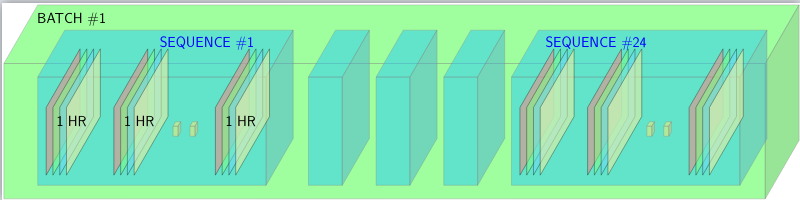
\includegraphics[scale=0.6]{ChapterX_Results_and_Conclusion/computational_experiments/temp_input_volume.png}
    \caption{Detailed sketch of the input volume to the $ConvLSTM-B_{10}-SL_{24}-32-3\times3-32-3 \times3$-model. Showing the content of the two first sequences in the first batch.}
    \label{fig:input_volume_conv_lstm}
\end{figure}

To explore the importance of spatial information from neighboring pixels the $ConvLSTM-B_{10}-SL_{24}-32-1\times1-32-1 \times1$-model was trained and compared to the best model. As expected, this model has a higher loss than the architecture trained using a $3\times 3$. This is shown in Table \ref{tab:convlstmLoss} summarizing the losses for all models in this study. \textbf{Denne figuren ser ut til å ha trent en bra sekvens i appendixen, se figure \ref{fig:timelapse_1x1}.}
%you can see it has the worst Test loss among the trained models. This indicate that information from adjacent pixels is useful. Its necesarry to mention that there is a significant difference between a \acrshort{ar}-model and a \acrshort{convlstm}-model with $1\times 1$ kernel and that is that the \acrshort{ar}-model train a different weight in all pixels, while the \acrshort{convlstm}-model utilize the same weights over the entire grid. 
%Not suprising ths that the number of parameters increase as the kernel increasse. 
%\clearpage
%\cleardoublepage

\subsection{Temporal Performance}
This section contains the evaluation of the $ConvLSTM-B_{10}-SL_{24}-32-3\times3-32-3 \times3$, $AR-B-L_5$ and \acrshort{era5} against \acrshort{ecc}. The metric used is \acrshort{mae} and the period is from 01.01.2014 to 31.12.2018. In making this comparison, please keep in mind that the \acrshort{ar}-model is optimized to fit and should be evaluated on its ability to predict one timestep. The \acrshort{convlstm}-model is trained and evaluated on its ability to fit a sequence of 24-hours.\textbf{ Some of the dependent variables to the parameterization in \acrshort{era5} is assimilated against a lot of observations, including radiance's from \acrlong{msg}} \cite{ERA52020}.

Figures \ref{fig:MAE_era}, \ref{fig:MAE_convlstm} and \ref{fig:MAE_AR} display the temporal skill of the parameterization. % on the task of predicting the cloud fraction cover in \acrshort{ecc}. 
%They scales are different in all the plots, and 
%%%%%%%%%%%%%%%%%%%%%%%%%% Trude du kom så langt
They show different regional biases. All models show clear distinction between land and ocean, the outline of Europe and North Africa is clearly visible.
As a whole the \acrshort{era5} have a more spotted pattern than the others. All models get a high skill in the Atlantic off coast of Spain and France. The same pattern can be found in Figure \ref{fig:deviation_sp} showing the standard deviation in surface pressure, but its most like not related.

The regions of low biases in Figures \ref{fig:MAE_AR} and \ref{fig:MAE_convlstm} are the same regions exhibiting a low mean and median cloud cover as shown in Figure \ref{fig:all_stats_tcc}.

Both these representations of \acrshort{cfc} have trouble with the Nile Delta. This doesn't not seem to be the case for $AR-B-L_5$. The correlation between \acrshort{ecc} to relative humidity is high compared to adjacent regions, as shown in Figure \ref{fig:correlation_tcc_vs_envio}. It is also worth mentioning that the bias and weight for $r$ is high in this region, which might explain the superior performance of \acrshort{ar}.
%%%%%%%%%%%%%%%%%%%%%%%%%%%%%%%%%%%%%%% Commenting on spatial patterens
\begin{figure}[ht]
    \centering
    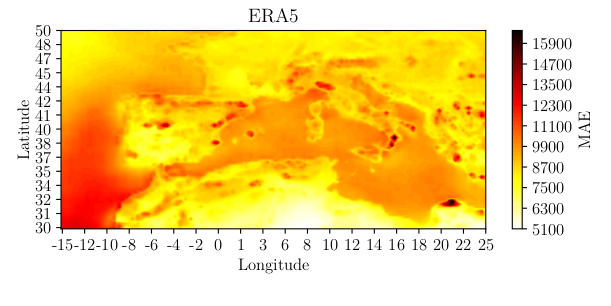
\includegraphics{python_figs/mae_era_vs_target_test_period_2014_to_2018.png}
    \caption{Evaluation of the parametrization in ERA5.}
    \label{fig:MAE_era}
\end{figure}
\begin{figure}[ht]
    \centering
    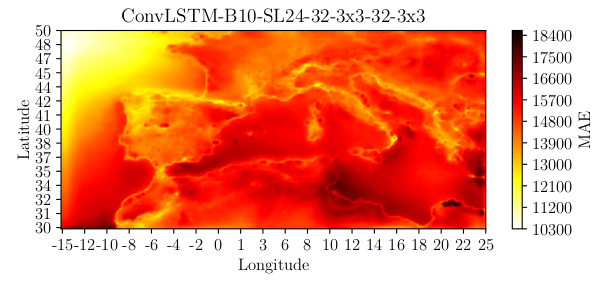
\includegraphics{python_figs/mae_convlstm_vs_target_test_period_2014_to_2018.png}
    \caption{Evaluation of the parameterization made by the $ConvLSTM-B_{10}-SL_{24}-32-3\times3-32-3 \times3$-model.}
    \label{fig:MAE_convlstm}
\end{figure}
\begin{figure}[ht]
    \centering
    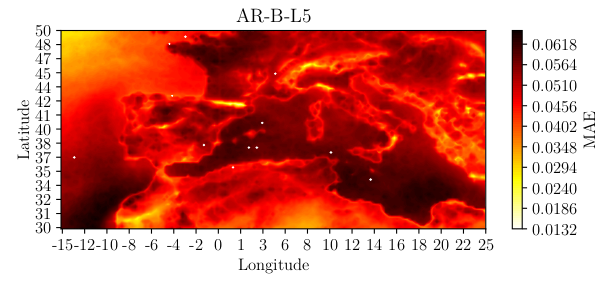
\includegraphics{python_figs/mea_best_ar_model_tcc_L5_in_folder_AR-B-L5.png}
    \caption{Evaluation of the parameterization made by the $AR-B-L_5$-model. The white dots visible is in total 12/13041 regression model having numerical issues related to non-invertable matrices.}
    \label{fig:MAE_AR}
\end{figure}

%%%%%%%%%%%%%%%%%%%%%%%%%%%%%%% Commenting on accumulated score 
%Table \ref{tab:tot_mae_score} summarise the \acrshort{mae} over the entire domain. Keep in mind that these number are not directly comparable, ERA5 is assimilated, its a forecast rerun and bias corrected against observations. The \acrshort{convlstm}-model use the reanalysis data (environmental variables only) at each timestep to predict sequences of cloud cover. The ar model use the target at previous timesteps and reanalysis data 

%%%%%%%%%%%%%%%%%%%%%%%%%%%%%%% Mention nan values in 
Unfortunately it was not recognized before later in this study that 
some models issues when training. Half of these problems are numerical issues related to matrix inversions and the other half is related to corrupt files. It is reason to believe this occurred during training since other configuration have results for all pixels. The temporal performance of other \acrshort{ar}-models can be found in the Appendix \ref{app:mae_plots}.

%%%%%%%%%%%%%%%%% OK OG PÅ RETT PLASS
Table \ref{tab:tot_mae_score} summarize the spatially averaged performance of the models. These results indicate that the overall best parameterization is made by the $AR-B-L5$-model. %This comparison is is a bit misleading since its evaluated on its ability to predict one time step ahead, which is a lot simpler task, than \acrshort{convlstm}-model, which is trained to predict 24 hours. 
\begin{table}[]
    \centering
    \begin{tabular}{cccc}
    \multicolumn{1}{c}{\textbf{}} & \textbf{ERA5} & \multicolumn{1}{c}{$\mathbf{AR-B-L_5}$} & \multicolumn{1}{c}{\textbf{$\mathbf{ConvLSTM-B_{10}-SL_{24}-32-3\times3-32-3\times3}$}} \\ \hline
    \textbf{MAE} & 0.20386 & 0.48502 &  0.33622 \\ \hline

    \end{tabular}
    \caption{\acrshort{mae} for the different cloud fractional cover parameterizations. }
    \label{tab:tot_mae_score}
\end{table}

\subsection{24-hour Cloud Cover Forecast}
%$AR-B-L_5$ $ConvLSTM-B_{10}-SL_{24}-32-3\times3-32-3 \times3$
This section provides a visual comparison of the $AR-B-S-L5$-model, $ConvLSTM-B_{10}-SL_{24}-32-3\times3-32-3 \times3$-model, ERA5 against \acrshort{ecc} on their ability on forecasting cloud cover 24-hours starting from January 2\textsuperscript{nd} 2014.

Figure \ref{fig:pred_sequence} shows the first six hours of the evolution cloud cover for the different models. The forecast produced by the different models are presented in their own column and the time progress down the rows. The 24-hour forecast is split into four figures and the full series is presented in Appendix \ref{app:pred_sequence}. 

%%%%%%%%%%% Presenter det du ser i en og en kolonne åså oppsmmerer du til slutt.
%%%%%%%%%% ERA5
\acrshort{era5} shows the most resembles to \acrshort{ecc}. This is not suprising since its the most complex parameterization included in this study, see Section \ref{sec:era5_param} for more details. \acrshort{era5} distribute the cloud over the same regions, but it has smoother transitions between cloudy and non-cloudy areas, which leads to a reduces total cloudyness compared to \acrshort{ecc}.

%%%%%%%%%%%%%%%%%%%%% CONVLSTM
There are few cloud present in the first few hours of the \acrshort{convlstm}-produced forecast. The cloud fractional cover developed slowly. From nine o'clock onwards, there is a significant overcast situation developed over parts Europe and Egypt. In general the forecast is a lot blurrier than \acrshort{ecc}. The time delay, present in the start of the forecast, may be explained by the fact that the forecast is not initiated with a cloud cover, only the environmental variables. Requires a few timesteps to spin-up/ develop the cloud cover.
%\textbf{Timedelay I guess this sorta makes sence since its not initiated with any cloud cover its needs a spin up}
% The outline of Europe is clearly visible.

%%%%%%%%%% AR
At first sight, the $AR-B-L_5$ appear to be very sensitive to the initial conditions. The first hour is a remarkable match, the following hours are not. It looks like the model creates a less cloudy copy of itself and present it as the next prediction. Near the end of the forecast, almost all clouds have dissipated leaving a few in Europe. This ``plagarims'' is most likely be caused by the weights of $L_1$ being close to $0.9$ as shown in Figure \ref{fig:weights_best_model}. The forecast is shown in isolation in Figure \ref{fig:timelapse_ar} and the spatial averaged cloud cover is included in the title. In the start of the forecast is has $0.6732$ which is reduced to $0.3676$ after 24-hours.
%%%% TARGET PREDICITON ERA5
\begin{figure}[ht]
    \centering
    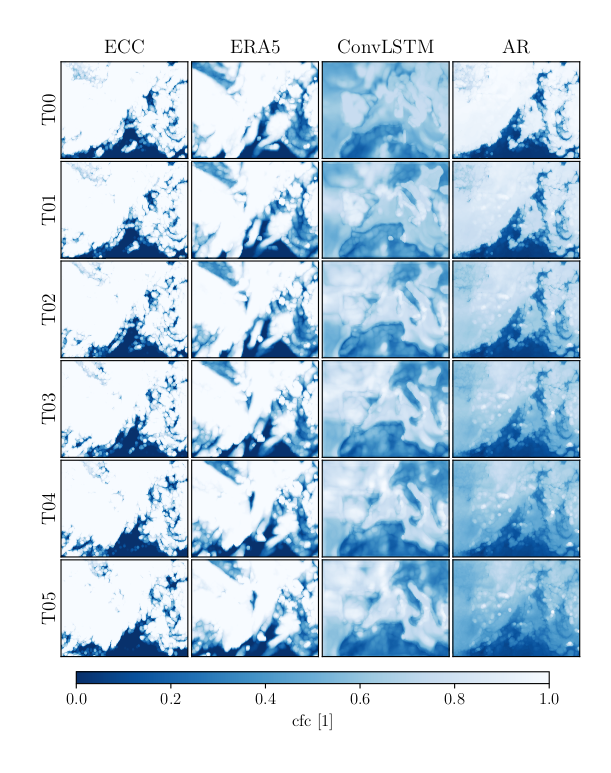
\includegraphics[sale=0.1]{python_figs/comparing_seq_part_1_of4_jan2.png}
    \caption{First six hours of a 24-hours forecast. The full forecast can be found in Appendix \ref{app:pred_sequence}.}
    \label{fig:pred_sequence}
\end{figure}

The displayed sequence predicted by $ConvLSTM-B_{10}-SL_{24}-32-3\times3-32-3 \times3$-model contain no out of sample values, but it is worth mentioning that for the entire period $0.5\%$ of the values produces are below zero, the lowest being -1, non above 1. 
%17140/3129840 = 0.005476318278250646

%%%%%%%%%%%%%%%%%%%%%%%%R und av med oppsummering av MAE table og 
Table \ref{tab:24hr_mae_score} shows the skill of the different models on predicting this 24 hours sequence. $ConvLSTM-B_{10}-SL_{24}-32-3\times3-32-3\times3$ rank highest having a score of 0.20386, ERA5 rank second with  $0.33622$ and $AR-B-L_5$ last with  $0.48502$. Note that a mean deviation of 0.46 is quite large when the data in question vary from 0 to 1. 
\begin{table}[]
    \centering
    \begin{tabular}{cccc}
    \multicolumn{1}{c}{\textbf{}} & \textbf{ERA5} & \multicolumn{1}{c}{$\mathbf{AR-B-L_5}$} & \multicolumn{1}{c}{\textbf{$\mathbf{ConvLSTM-B_{10}-SL_{24}-32-3\times3-32-3\times3}$}} \\ \hline
    \textbf{MAE} & 0.392 & 0.485 & 0.278 \\ \hline
    \textbf{MIN} & 0.0 & 0.004 & 0.0 \\ \hline
    \textbf{MAX} & 1.0 & 1.028 & 1.0 \\ 
    \end{tabular}
    \caption{\acrshort{mae}, minimum and maximum values for the 24-hour forecast period of 2\textsuperscrip{nd} January 2014. }
    \label{tab:24hr_mae_score}
\end{table}

The minimum value in this prediction (AR) is positive, and the maximum is $1.028$. It a hundred and three percent cloudy. 

To the authors surprise the Figure \ref{fig:timelapse_1x1} appears to have a more realistic cloud forecast than \ref{fig:timelapse_3x3}, which is surprising - It has a lower score.

A comment on the out-of-sample value used to fill the gaps.
\textbf{Du kan kommentere at selv om missing values ble fylt i med out of sample verdien 1.5, produserer ikke consltms noen out of sample positive veridier}

%%%%%%%%%%%%%%%%%%% Practical implications
\subsection{Practical implications} \label{sec:practical_implications}
%It is necessary to have a understanding of the needs of the end product before conducting large machine learning projects. Answering questions like: What will it be used for and how can it be implemented in useful way?
A major downside of the data driven learning approach is the rigid resolution. A trained model can only be used on similar problems, with the same spatiotemporal resolution. For applications like climate models, output comes in a wide range of different resolutions. Before implementing the finished product in a new model of a different resolution, it would need to be retrained on the resolution of the climate model under development. This process involves both remapping of the dataset and retraining the model at the correct resolution. This is a time consuming process involving finding a new set of hyperparameters suitable for the new resolution. % It essentially means starting over.
%TS: Er ikke dette noe som bør undersøkes i fremtidige studier? M.a.o., er det alltid nødvendig "å starte om igjen" hvis oppløsningen endrer seg? Og hvor forskjellig må oppløsningen være for at det skal være nødvendig?

Once trained on global climate datasets, machine learning models provide fast results even for complex parameterization, which is what makes them suitable for the application of climate modelling. Most machine learning packages are developed using Python. \acrfull{esm} are increasingly also implemented in python. Methods for including the trained parameterizations need to be developed to further explore the potential of machine learning for climate modeling in the future.
%Uten transformasjon er det kanskje naturlig å sette prediksjoner < 0 til 0 og alle > 1 til 1. 

%%%%%%%%%%%%%%%%%%%%%%%%% Summary

\subsection{Summary} \label{sec:summary_num}
%%%%%%% Rart med summary her rett før conclusion?
In this section %X antall modeller har blitt trent og evaluert på ecc. Nevn train test split?
two types models have been trained and evaluated on task of predicting cloud cover in \acrshort{ecc}.
Several configuration of each kind was considered. The best each was compared against \acrshort{era5} on producing a 24-hour cloud forecast.

As a reference \acrshort{mae}, \acrshort{era5} had $0.20386$. 
The best \acrshort{ar}-configuration is $AR-B-L_5$ \acrshort{mae} of $0.04901$. This is incrementally better than other $AR-B$-configurations by varying on number of lags. Unfortunately, the ``copy''-effect renders the model unfit to producing a realistic cloud cover further ahead in time than one hour. 
%overfittet to the cloud cover at previous timesteps. Consequently its unable to produce sequences, it simply produce dampened copies of the initial cloud cover. The \acrshort{ar}-models might be to simple for performing this task? 

$ConvLSTM-B_{10}-SL_{24}-32-3\times3-32-3\times3$ was the best \acrshort{convlstm}-configuration. 
Measured over the entire test period i did rather badly, having a \acrshort{mae} of $0.48502$. It showed skill when producing the forecast, a few hours into the forecast it was able to reproduce the cloudy regions in \acrshort{ecc}.  

%%%%%%%%%%%%%%%%%%%%% Kanskje med conclusion mat


% NOTES IN CASE I FORGET WHERE THE NUMBER CAME FROM
%\begin{enumerate}
%    \item Radar Echo: 1 sequence is 20 Frame one frame is 100x100. Train seq. 8148, 2037 for valid and 2037 for test. 
%    \item 1629600000 Num Train, 407400000 Num Valid and 407400000 num Test
%    \item KDD Weather data 21x31x5 365.25*24 (Train), 30*24(Valid, test)
%    \item 28513800 (Train) samples, 2343600 (Valid, Test)
%\end{enumerate}
%\textbf{Ønsker å understreke dette for det er }
%It is more difficult to train a models on a larger amount of data. 

